\documentclass[11pt,a4paper,twoside,openright,cleardoublepage=plain]{scrreprt}

\usepackage{bftn}

\usepackage[OT1]{fontenc}
\usepackage[utf8]{inputenc}

\usepackage{graphicx}
\usepackage{color}

\usepackage[english]{babel}
\usepackage[clearempty]{titlesec}
\usepackage{xspace} % because I'm lazy -- Simu

\usepackage[dvips, bookmarks, colorlinks=false, pdfborder=(0 0 0),
	    pdftitle={A Messaging Interface to Disks},
	    pdfauthor={Manuel Stocker, Mark Nevill, Simon Gerber},
	    pdfsubject={A Message Interface to Disks},
	    pdfkeywords={Barrelfish, AHCI, MPI}]{hyperref}

\usepackage{listings}

\usepackage{algorithmic}
\usepackage[chapter]{algorithm}

\usepackage[acronym,shortcuts,nonumberlist,toc]{glossaries}
\glossarystyle{long3col}
\makeglossaries

\usepackage{hyphenat}

\lstset{basicstyle=\ttfamily,columns=fixed,basewidth=0.5em,showstringspaces=false,language=c,captionpos=b,tabsize=4}

\usepackage{nameref}
\newcommand{\longref}[1]{\autoref{#1},~\nameref{#1}}


\title{A Messaging Interface to Disks}
\author{Manuel Stocker, Mark Nevill, Simon Gerber}
\tnnumber{015}
\tnkey{Disk Driver Architecture}


\begin{document}

\newacronym{ahci}{AHCI}{Advanced Host Controller Interface}
\newacronym{sata}{SATA}{Serial ATA}
\newacronym{pata}{PATA}{Parallel ATA}
\newacronym{ata}{ATA}{AT Attachment}
\newacronym{atapi}{ATAPI}{AT Attachment Packet Interface}
\newacronym{acs}{ACS}{ATA Command Set}
\newacronym{lba}{LBA}{Logical Block Address}
\newacronym{hba}{HBA}{Host Bus Adapter}
\newacronym{fis}{FIS}{Frame Information Structure}
\newacronym{rfis}{RFIS}{Received FIS}
\newacronym{fat}{FAT}{File Allocation Table}
\newacronym{cam}{CAM}{Common Access Method}
\newacronym{sim}{SIM}{SCSI Interface Module}
\newacronym{prd}{PRD}{Physical Region Descriptor}
\newacronym{fsis}{FSIS}{Filesystem Information Sector}
\newacronym{bar}{BAR}{Base Address Register}
\newacronym{pci}{PCI}{Peripheral Component Interconnect}
\newacronym{ascii}{ASCII}{American Standard Code for Information Interchange}
\newacronym{scsi}{SCSI}{Small Computer System Interface}
\newacronym{idc}{IDC}{Inter-Domain Communication}
\newacronym{rpc}{RPC}{Remote Procedure Call}
\newacronym{vfs}{VFS}{Virtual Filesystem}
\newacronym{piix}{PIIX}{PCI IDE ISA Xcelerator}
\newacronym{ich}{ICH}{I/O Controller Hub}
\newacronym{dma}{DMA}{Direct Memory Access}
\newacronym{lru}{LRU}{Least-recently used}
\newacronym{skb}{SKB}{System Knowledgebase}
\newacronym{ncq}{NCQ}{Native Command Queueing}


\maketitle

\begin{abstract}
This lab project introduces an \acs{ahci} driver and associated \acs{ata}
primitives to Barrelfish\footnote{\url{http://www.barrelfish.org}}. Interfacing
disks is implemented in a library that communicates with a management service.
To enable integration of multiple controllers offering access to
\acs{ata}/\acs{atapi}-based devices, Flounder modifications including a backend
for \acs{ahci} are proposed. This project also provides a basic analysis of the
driver's performance characteristics. To demonstrate usage, a simple testcase,
a FAT filesystem implementation and a simple block device filesystem are
introduced.
\end{abstract}


\tableofcontents

\chapter{Introduction}
The \ac{ahci} is a standard by Intel that defines a common API for \ac{sata}
and SAS host bus adapters. In order to provide backwards-compatibility,
\ac{ahci} specifies modes for both legacy IDE emulation and a standardized
\ac{ahci} interface. 

\ac{ahci} only implements the transport aspect of the communication with
devices. Commands are still transferred as specified in the \ac{ata}/\ac{atapi}
standards.

\section{ATA/ATAPI/SATA}

The \ac{ata} standard specifies an interface for connecting several types of
storage devices, including devices with removable media. \ac{atapi} provides an
extension to allow \ac{ata} to transmit \acs{scsi} commands.

Commands that can be sent to \ac{ata} devices are specified in the \ac{acs}
specifications. Commands in particular interest for this lab project are the
\texttt{IDENTIFY}, \texttt{READ DMA}, \texttt{WRITE DMA} and \texttt{FLUSH
CACHE} commands.

The way these commands are sent to the device is specified in the respective
specification, for example the \ac{sata} or \ac{pata} specifications.

\subsection{SATA}

The \ac{sata} standard specifies the layout of the command \acp{fis} that
encapsulate traditional ATA commands as well as all the lower layers of the
interface to the disk, such as the physical layer.

Figure \ref{fig:h2d_fis} shows the structure of an example \ac{fis}. A Host to
Device Register \ac{fis} can be used to send commands to the disk. The command
value is specified by \ac{ata}. The \ac{fis} contains additional values such as
\ac{lba} and sector count.

\begin{figure}[ht]
\centering

\includegraphics[width=.7\textwidth]{h2d_fis.pdf}
\caption{Host to Device Register FIS \cite[p.~336]{sata_2.6}}
\label{fig:h2d_fis}
\end{figure}

\section{AHCI}

\subsection{Memory Registers}

While the \acs{pci} base address register 0-4 may contain pointers to address
spaces for legacy IDE emulation, \ac{bar} 5 contains the address of the
\ac{hba}'s memory mapped registers. As shown in figure \ref{fig:hba_mem}, this
address space is divided into two areas: global registers for control of the
\ac{hba} and registers for up to 32 ports. A port can be attached to either a
device or a port multiplier. In this lab project, we focus on device handling
and ignore port multipliers.

\begin{figure}[ht]
\centering
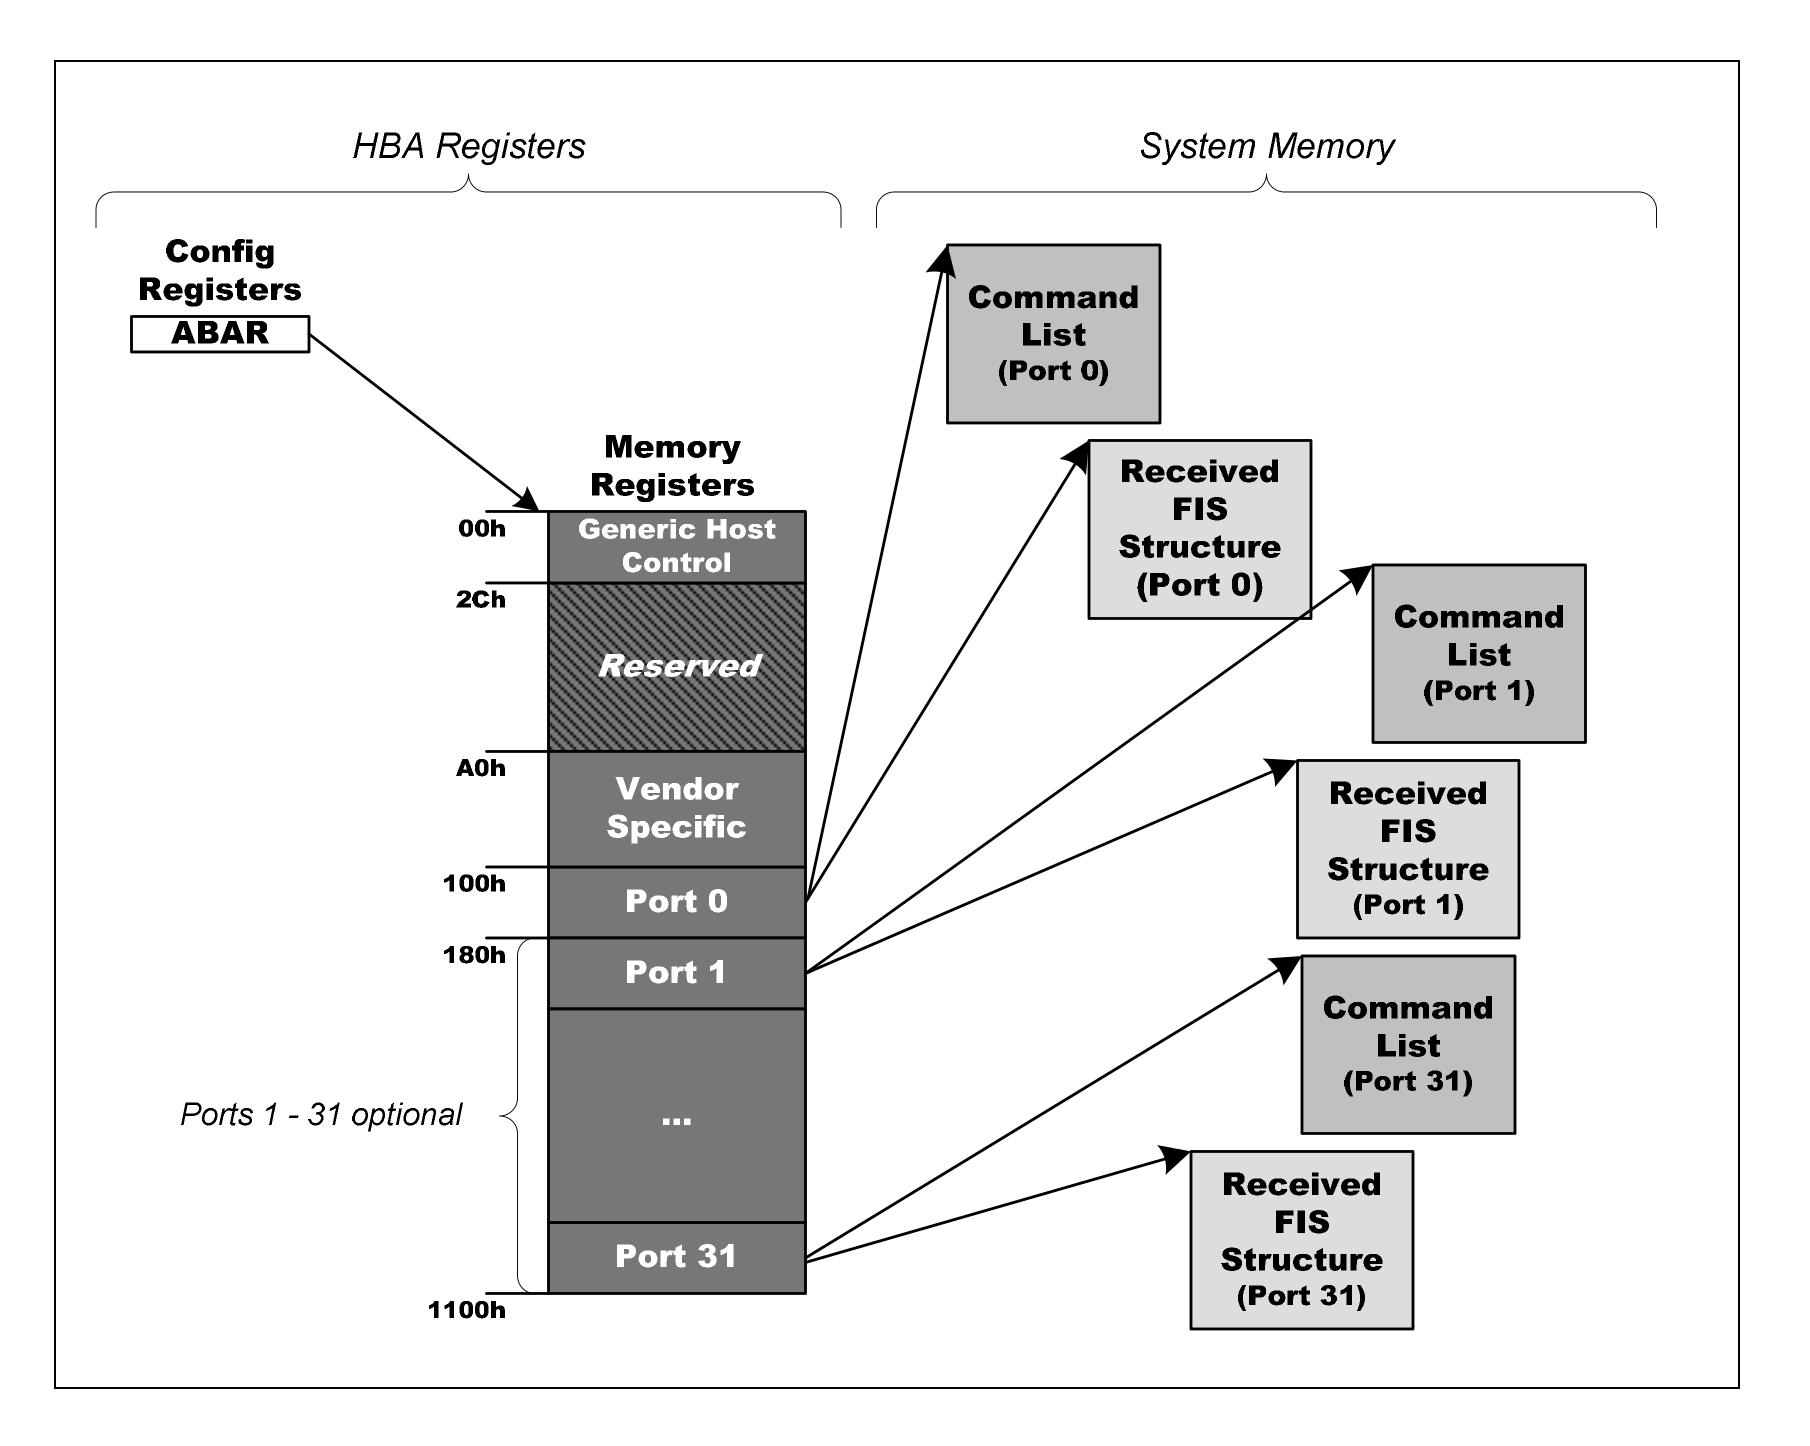
\includegraphics[width=.7\textwidth]{hba_mem.png}
\caption{HBA Memory Space Usage \cite[p.~33]{ahci_1.3}}
\label{fig:hba_mem}
\end{figure}

Every port area (\autoref{fig:port_mem}) contains further control registers and
pointers to the memory regions for the command list and receive \ac{fis} area.
Each of these pointers is a 64-bit value (32-bit for \acp{hba} that don't
support 64-bit addressing) stored in two port registers.

\begin{figure}[ht]
\centering

\includegraphics[width=.9\textwidth]{pmem_overview.pdf}
\caption{Port System Memory Structure adapted from \cite[p.~34]{ahci_1.3}}
\label{fig:port_mem}
\end{figure}

\subsection{Received FIS Area}

The received \ac{fis} area serves as an area where copies of the \acp{fis}
received from the device are stored. The \ac{hba} will copy all incoming
\acp{fis} to the appropriate region of the \ac{rfis} area. If the \ac{hba}
receives an unkown \ac{fis} it is copied to the Unknown \ac{fis} region if it
is at most 64 bytes long. If the \ac{hba} receives an unknown \ac{fis} that is
longer than 64 bytes, it will be considered illegal.

\begin{figure}[ht]
\centering
\includegraphics[width=.8\textwidth]{rfis_area.pdf}
\caption{Received FIS Organization, adapted from \cite[p.~35]{ahci_1.3}}
\label{fig:rfis_mem}
\end{figure}


\subsection{Commands}

A command list (\autoref{fig:command_list}) contains 32 command headers, which
each contain the metadata for a single command.

Commands can be issued to the device by constructing a command header
containing a reference to a command table and further metadata for the command
to be issued.

\begin{figure}[ht]
\centering
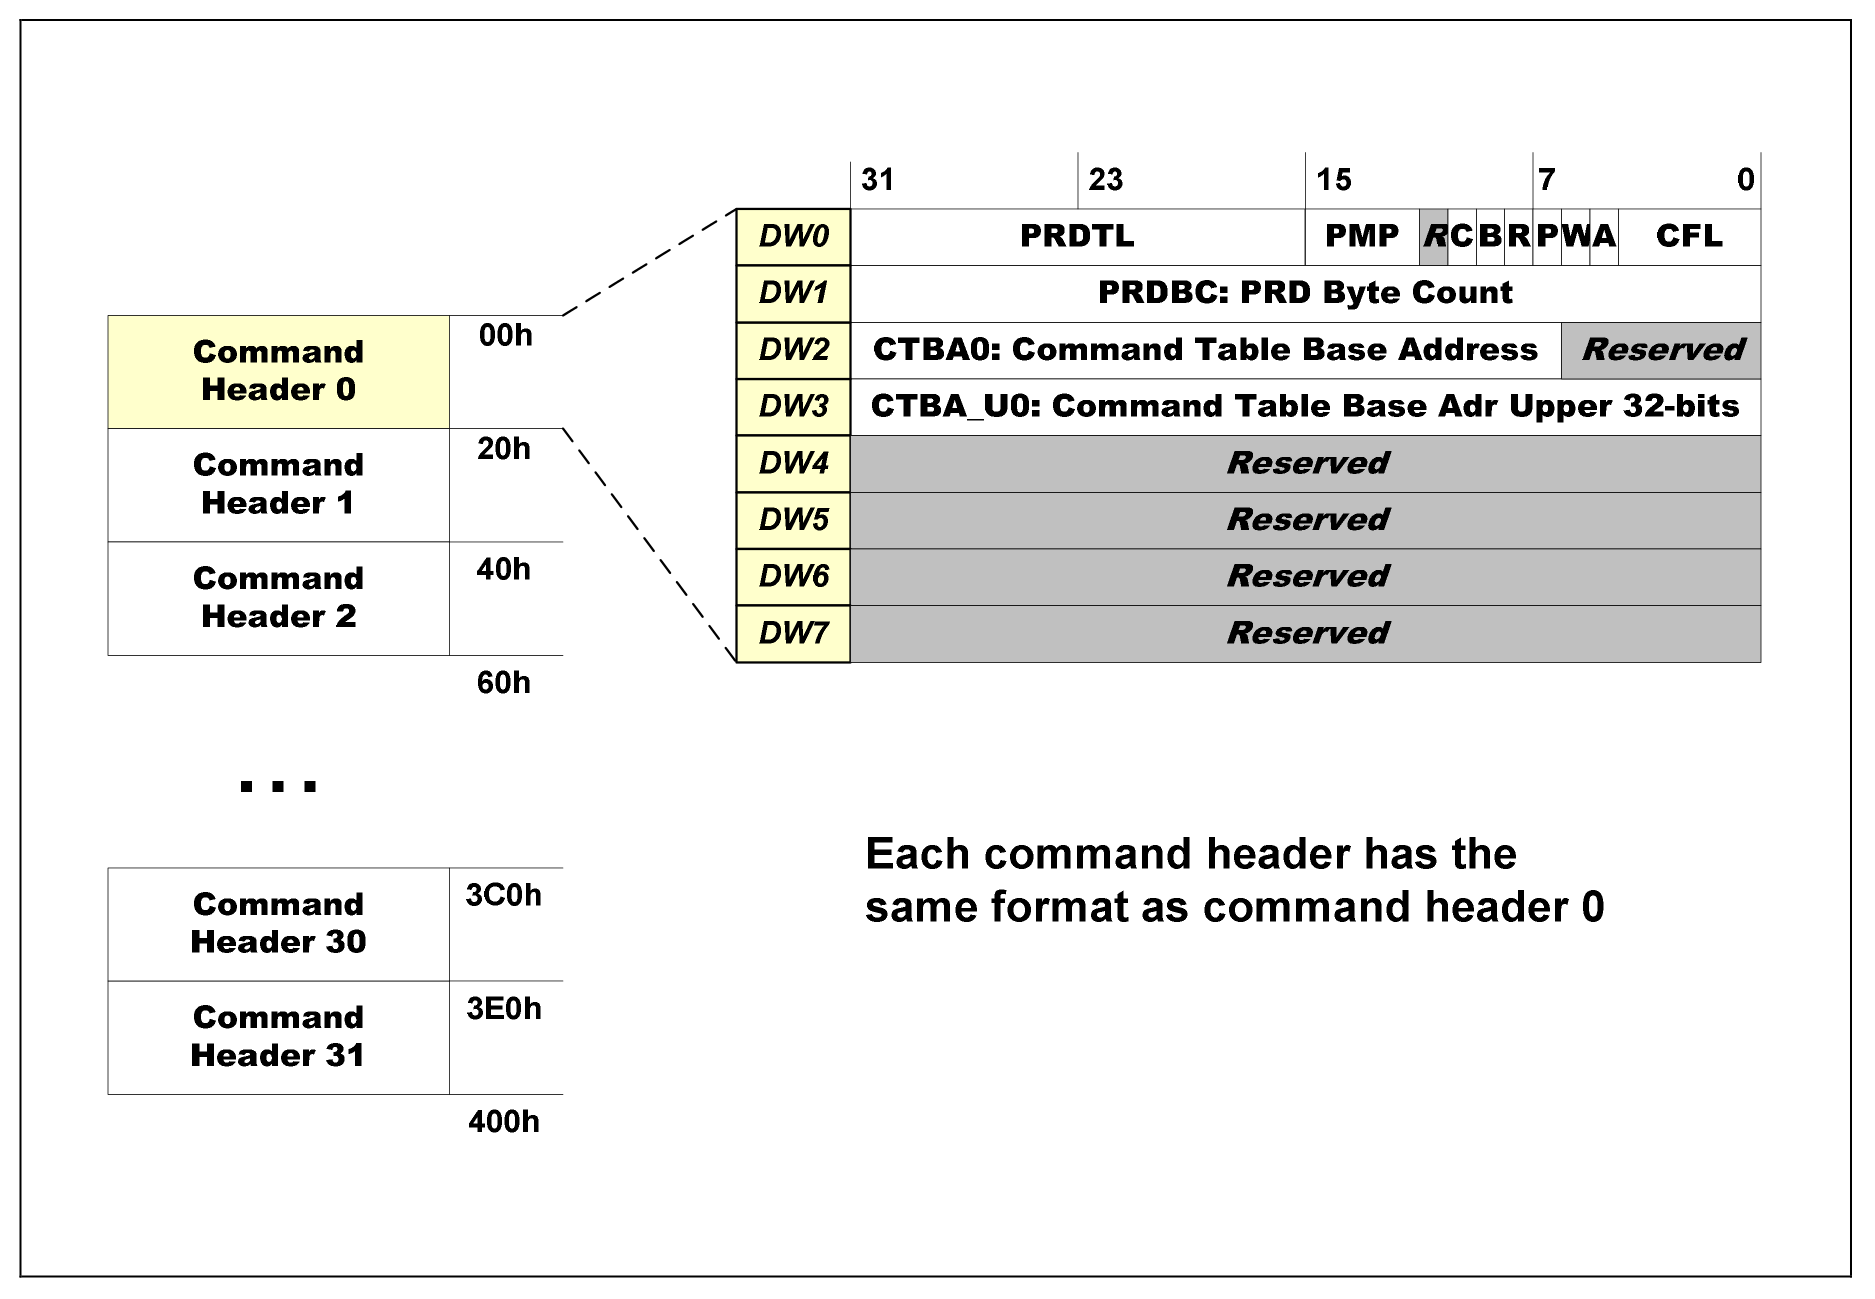
\includegraphics[width=.8\textwidth]{command_list_structure.png}
\caption{Command List Structure \cite[p.~36]{ahci_1.3}}
\label{fig:command_list}
\end{figure}

The command table (\autoref{fig:command_table}) contains the command \ac{fis}
itself and an optional number of physical region descriptors specifying chunks
of main memory in form of a scatter-gather list.

\begin{figure}[ht]
\centering
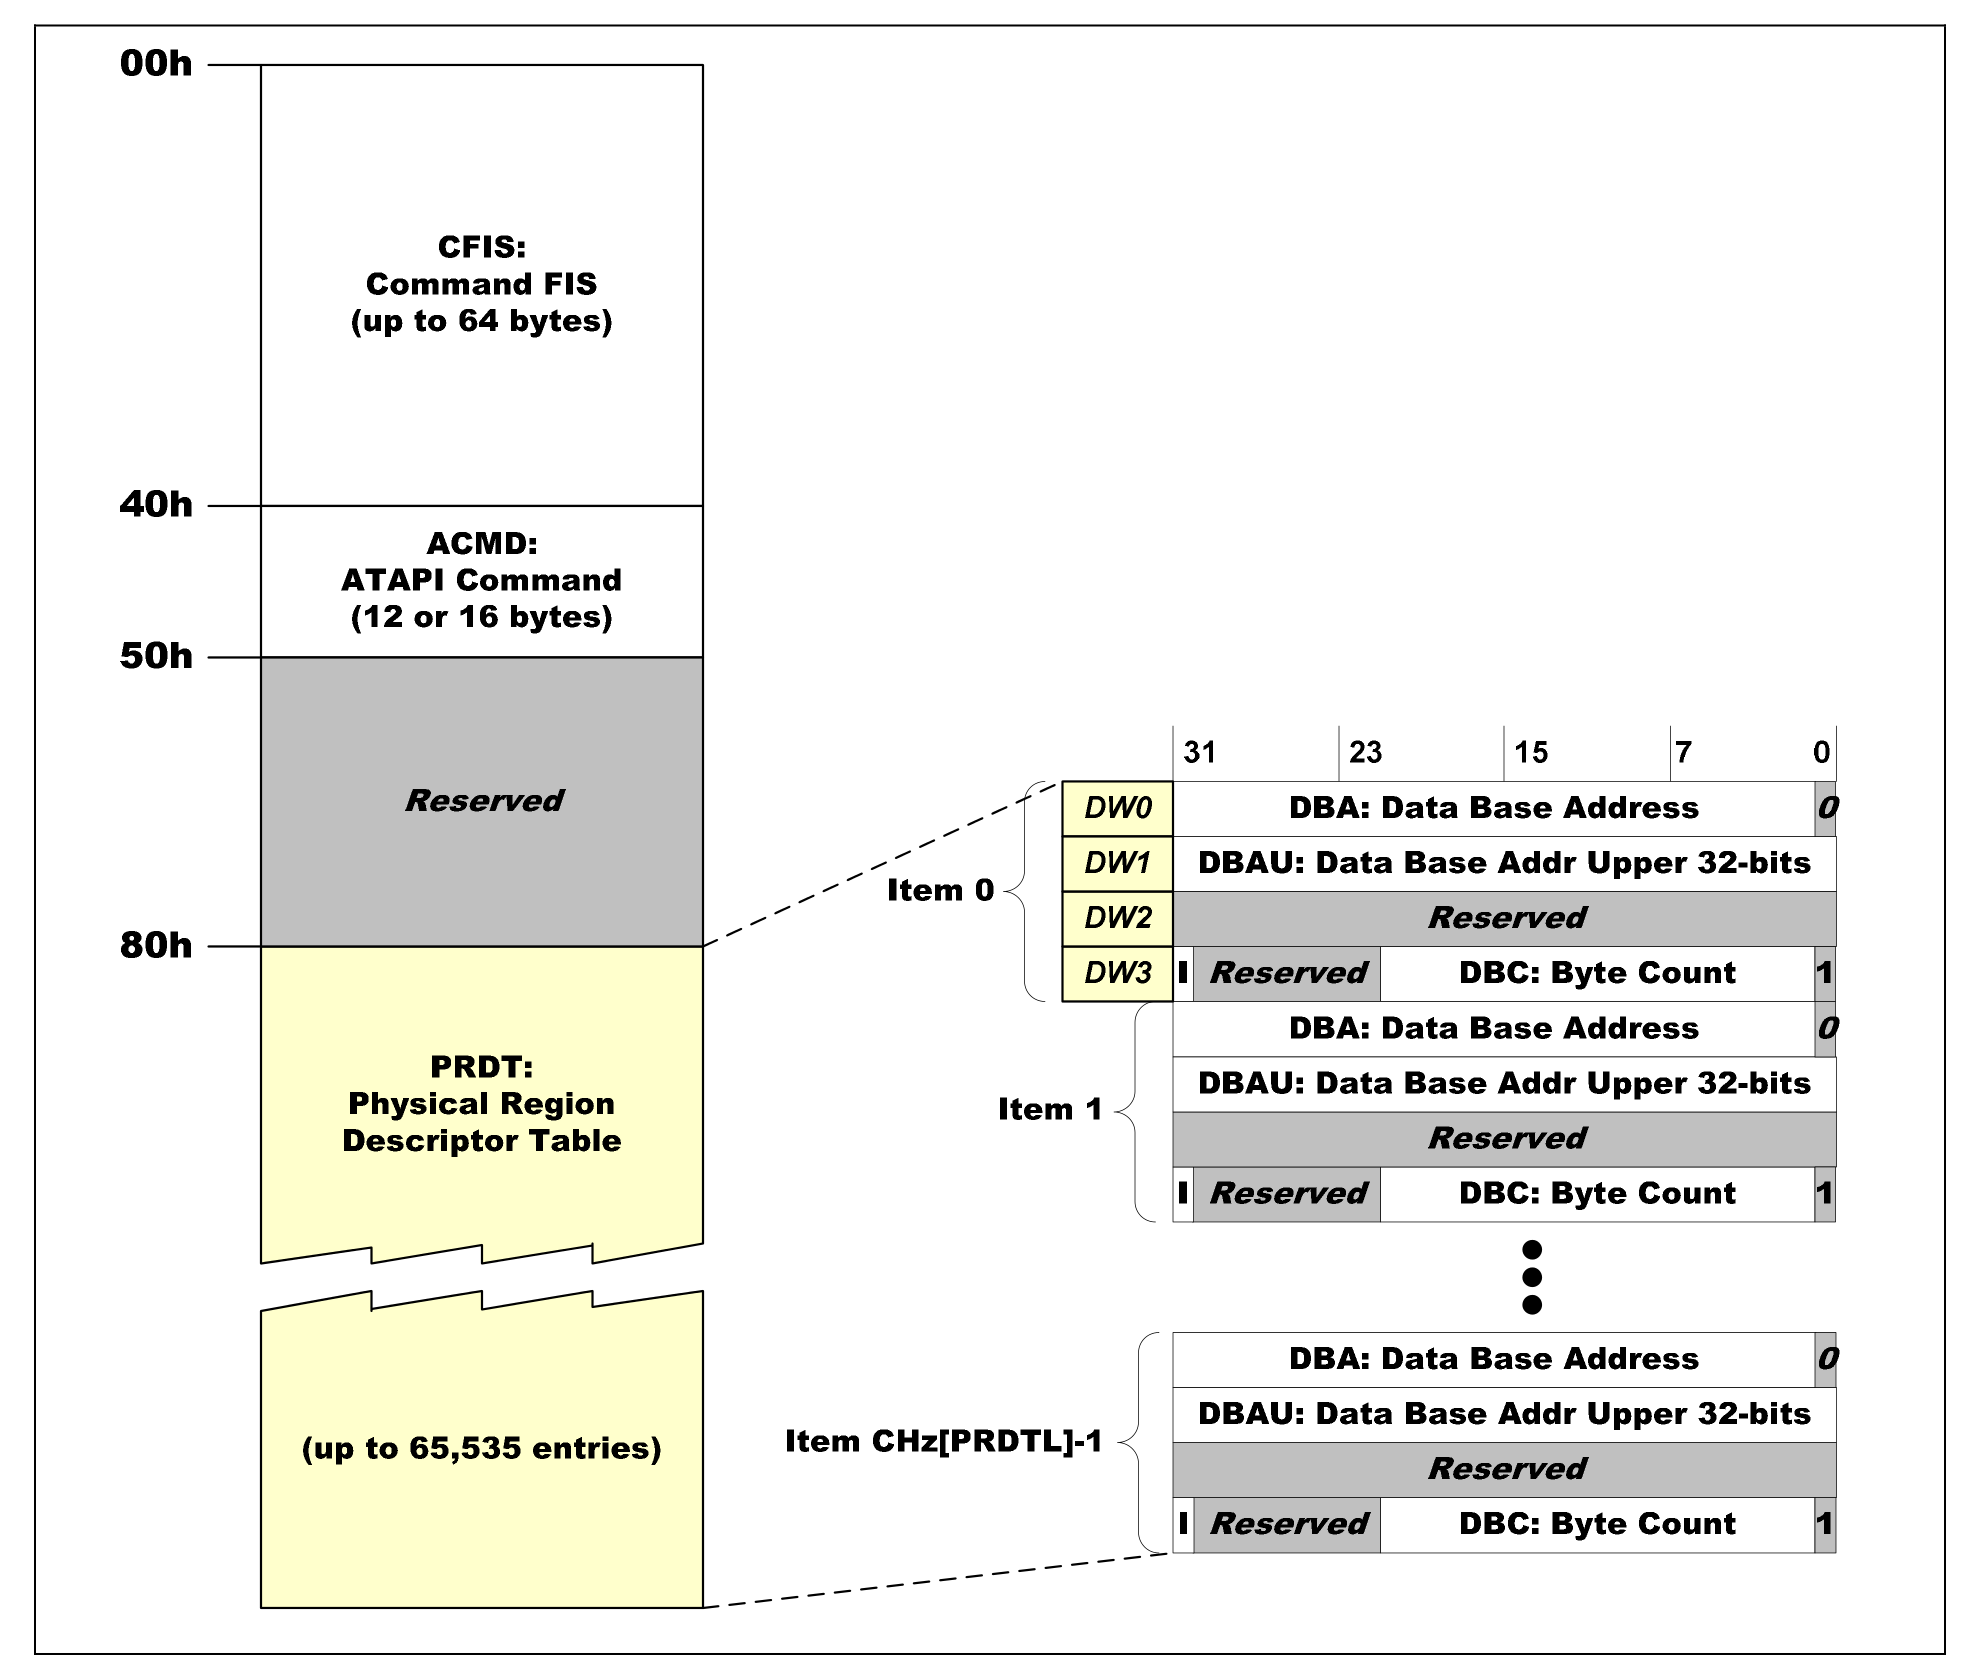
\includegraphics[width=.8\textwidth]{command_table.png}
\caption{Command Table \cite[p.~39]{ahci_1.3}}
\label{fig:command_table}
\end{figure}

Commands are issued by setting the corresponding bit in the command issue
register. Upon command completion, the bit is cleared and if enabled, an
interrupt is triggered.



\chapter{Related Work}
\section{Other OSes}

Most Unix-derived Operating Systems (Linux, BSD flavours, OpenSolaris, etc)
integrate their \ac{ahci} subsystem into a larger disk subsystem with support
for IDE disks, \ac{sata} disks (via \ac{ahci}), CDROM/DVD drives, and also
floppy drives.

This larger disk subsystem often utilizes a general buffer layer which the OS
kernel provides to its subsystems. Furthermore most Unix derivates -- due to
their essentially monolithic nature -- couple the different layers of their
disk subsystems (transport layer, message format and disk commands, e.g.
\ac{ahci}, \ac{sata} and \ac{ata} respectively) using function pointers and
most of them have in-kernel structures that describe commands that are issued
to the disk in a message format and transport agnostic way. This makes those
systems relatively easy to extend by adding a new layer implementations (e.g.
when \ac{ahci} was first implemented a few years ago, it was as simple as
providing a new transport layer implementation for disks attached to \ac{ahci}
controller).

\subsection{FreeBSD}

FreeBSD employs the \ac{cam}\footnote{FreeBSD \acs{scsi} Documentation can be
found under
\url{http://www.freebsd.org/doc/en_US.ISO8859-1/books/arch-handbook/scsi-general.html}}
framework to seperate implementation of the driver for the I/O bus from the
device driver for the attached device. Therefore, FreeBSD's \ac{ahci} driver is
realized as a \ac{sim} handling the I/O operations needed to get an \ac{ata} or
\acs{scsi} command to the device (transparently using the packet interface of
\ac{atapi}). Other aspects of the storage system, such as filesystem or disk
driver do not have to be modified.

\subsection{Linux}

Linux handles access to \ac{ata} devices with libATA\footnote{The libATA
Developer's Guide can be found under
\url{http://www.kernel.org/doc/htmldocs/libata.html}} which unifies interfacing
with \acs{scsi} and \ac{ata} based devices and adapters in a common API. libATA
can translate \acs{scsi} commands to \ac{ata} and vice-versa or simulate a
certain command if there is no translation possible.  Drivers for adapters only
need to implement hooks for basic device operations and communication.


\chapter{Design}
\section{Design Options}

In order to be able to register as a \acs{pci} device driver, some sort of
management process for receiving the interrupts is necessary. A management
process is also useful for device detection and initialization, providing the
system with an overall view of what devices are available.

Consumers of \ac{ahci}-related interrupts must register with the management
process so that interrupts may be forwarded. To provide clients with access to
different \ac{sata} devices, it makes sense to grant access to invidual
\ac{hba} ports, and similarly to forward all interrupts for a port to any
clients registered to that port.

However, in choosing the method of accessing the ports, a trade-off must be
made between security and performance. For example, by setting a suitable
address, another domain's memory can be written to disk, and then read back,
violating domain separation. To stop this from occuring, a central location
must check that all \acp{prd} reference memory which the client may access.

In such a design, all port memory access, including issuing of commands, would
happen via Flounder messages to the central daemon. The central daemon would
have to ensure that the client does not modify the command list or command
tables after they are checked, so the all these areas would have to be copied
into a memory area not accessible to the client.

To achieve optimal performance at the cost of security, each client must be
given full access to the port memory. Because this is usually within the same
page as the \ac{hba} memory, clients are able to access not just their own
port's registers, but all other ports' and the \ac{hba}'s registers as well.
Also, as described above, the client can access all memory with suitable
\acs{dma} commands.

\section{General Architecture}

\begin{figure}[ht]
\centering
\includegraphics[width=.9\textwidth]{architecture.pdf}
\captionof{figure}{Barrelfish AHCI subsystem architecture}
\label{fig:architecture}
\end{figure}

As shown in in \autoref{fig:architecture}, our message passing to disk has two
main parts: a management part and a communication part. The management part,
\emph{ahcid}, provides a system-wide authority over an \ac{ahci} controller.
The communication part, consisting of libahci (a low-level abstraction for
using an \ac{ahci} port) and the \ac{ata} message specification and translation
layer using Flounder, is used by all user-level code that wants to access a
disk to send and receive messages from a disk.

\section{ahcid}

ahcid exists as a central point of authority over an \ac{ahci} \ac{hba}. It is
responsible for \ac{hba} initialization, Interrupt handling and access
mediation.

\subsection{Operation}

ahcid ensures only one user can access an \ac{ahci} port at a time. Users can
open a port by sending an \acs{idc} message to ahcid. If no other user
currently owns the port, ahcid will provide a memory capability to the port's
memory registers.  The user is then able to use the port exclusively.
Interrupts generated by the port are handled by ahcid and dispatched to the
associated user via an \acs{idc} message. ahcid registers itself as PCI device
driver for certain \ac{ahci} chipsets.

\section{libahci}

libahci tries to hide the necessary bit-twiddling and \acs{dma} buffer
management for sending and receiving messages to a disk. Its interface
resembles a Flounder-generated interface and makes use of Barrelfish's
waitsets.

\section{Flounder Backend}

This lab project also contains a Flounder backend and Flounder modifications in
order to be able to specify \ac{ata} commands as message definitions. The
resulting interface can be used similarly to performing \acs{idc}.

\section{Implemented ATA Commands}

For our purposes (designing a messaging interface to disks) it was sufficient
to implement commands for reading and writing blocks to and from disks using
\acs{dma} (\ac{ata} commands {\tt READ DMA}, {\tt WRITE DMA}), inspecting the
disk ({\tt IDENTIFY}) and flushing the cache ({\tt FLUSH CACHE}). Due to the
Flounder layer in our system (specifically the \acs{ahci} backend) adding new
\ac{ata} commands is quite easy: just add the command you want in the \ac{ata}
interface specification.


\chapter{ahcid}
\label{chap:ahcid}

\section{Introduction}

\subsection{Public IDC Interface}

ahcid's design is modeled after netd. It has a small \acs{idc} interface that
facilitates user access to a port: when registering for a port, the user is
given the capability for the port registers. Interrupts are forwarded via
\acs{idc} messages.  Currently the interface also provides access to the {\tt
IDENTIFY} data of all available disks. This is useful to determine the type of
device and total disk space without having to open the port.

\begin{center}
\begin{minipage}{100mm}
\begin{lstlisting}[label={code:ahci_mgmt.if}, caption={ahci management Flounder
interface}]
interface ahci_mgmt "AHCI Management Daemon" {

    rpc list(out uint8 port_ids[len]);
    rpc identify(in uint8 port_id,
                 out uint8 identify_data[data_len]);

    rpc open(in uint8 port_id, out errval status,
             out cap controller_mem, out
             uint64 offset, out uint32 capabilities);
    rpc close(in uint8 port_id, out errval status);

    message command_completed(uint8 port_id,
                              uint32 interrupt_status);
};
\end{lstlisting}
\end{minipage}
\end{center}

\section{Initialization}

ahcid registers itself as a driver for the \ac{ahci} device class. Once the
init procedure is called, ahcid consults the received base address registers to
find the memory region used for the \acs{hba}'s registers.

As a first step, the \ac{hba} is reset in order to get to a known state. The
\ac{hba} is also put into \ac{ahci} mode. After the initial reset, ahcid
discovers the number of ports and detects which of them are implemented and
have a disk connected.  Discovered disks are assigned a system-wide unique port
id and are registered with the skb. For every disk, an \ac{ata} {\tt IDENTIFY}
command is sent to determine the disk's parameters. A copy of the {\tt
IDENTIFY} response is cached in ahcid for later use.

After all attached disks are initialized, ahcid exports the ahci management
interface, which clients can then use to register themselves for a single port.

\section{Interrupt Handling}

ahcid registers itself as an interrupt handler for the \ac{ahci} \ac{hba}
controller when calling \lstinline+pci_register_driver_irq+. The interrupt
handler extracts the current interrupt state of the controller from the device
memory and decides if the interrupt was triggered by the \ac{hba}. If the
interrupt was triggered by the \ac{hba}, the handler loops over all ports and
checks which ports received an interrupt and clears the port's interrupt
register. The \ac{hba}'s interrupt register is cleared after all port interrupt
registers have been cleared. At last, if a client is registered for a port that
has received an interrupt, ahcid sends a \lstinline+command_completed+ message
(\autoref{code:ahci_mgmt.if}) using the established \lstinline+ahci_mgmt+
interface. Clearing the interrupts before delivering the completion messages to
the respective users ensures that we do not miss interrupts that would be
triggered as a consequence of any commands issued in the command completion
handler. Missing any interrupts for further completions could deadlock a user
since we do not poll the port's state if no interrupts have been triggered.


\chapter{libahci}
\section{Introduction}

\newcommand{\libahci}{\lstinline+libahci+\xspace}

\subsection{Purpose}

The intent behind \libahci is to provide an easy-to-use low-level interface to
a single \ac{ahci} port. The main reason why such a library is desirable is to
be able to send arbitrary \ac{ata} commands via \ac{ahci} without having to
bother with the \ac{ahci} specification details.

\subsection{Design}

\libahci abstracts the low-level \ac{ahci} operations such as the writing to
memory mapped control registers of the \ac{hba}. It exposes an interface
similar to that of Flounder-generated interfaces to offer a familiar
environment for Barrelfish developers.  The library is also used for the
\ac{ahci} specific layer of the Flounder \ac{ahci} backend. It acts as a
central point for interfacing \ac{ahci} controllers.

Apart from handling the sending of \ac{ahci} formatted \ac{ata} messages,
\libahci also provides memory management for \acs{dma} regions.

\section{DMA Buffer Pool}

As all data transfers with \ac{ahci} as transport are done via \acs{dma}, we
need a mechanism to manage data buffers that are mapped non-cached. Because
Barrelfish does not have memory reclamation for raw frame allocation, we must
manage these buffers ourselves and have therefore implemented our own memory
subsystem in the form of a \acs{dma} buffer pool, which allows for \acs{dma}
buffer allocation and freeing.

The user has to call \lstinline+ahci_dma_pool_init+ to initialize the \acs{dma}
buffer pool. After that, calls to \lstinline+ahci_dma_region_alloc+ and
\lstinline+ahci_dma_region_alloc_aligned+ allocate buffers of the given size
rounded up to 512 bytes, and the latter aligns the base address such that {\tt
base \% alignment\_requirement == 0}. \lstinline+ahci_dma_region_free+ returns
the region it gets passed to the pool.

Additionally the buffer pool provides helper functions that facilitate copying
data in and out of a buffer (\lstinline+ahci_dma_region_copy_in+ and
\lstinline+ahci_dma_region_copy_out+).

\begin{center}
\begin{minipage}{54mm}
\begin{lstlisting}[caption={DMA region handle},label=code:reghandle]
struct ahci_dma_region {
    void *vaddr;
    genpaddr_t paddr;
    size_t size;
    size_t backing_region;
};
\end{lstlisting}
\end{minipage}
\end{center}

\begin{figure}[p]
\centering
\includegraphics[width=.85\textwidth]{dma_pool_design.pdf}
\caption{DMA Buffer Pool Design}
\label{fig:dma_pool_design}
\end{figure}

\subsection{Design}

The pool memory is organized in regions which are allocated and mapped using
\linebreak\lstinline+frame_alloc+ and \lstinline+vspace_map_one_frame+
respectively. The virtual and physical addresses of each of these regions are
stored in the fields \lstinline+vaddr+ and \lstinline+paddr+ of
\linebreak\lstinline+struct dma_pool+ (c.f.~\autoref{fig:dma_pool_design}). The
\acs{dma} buffer pool uses a doubly linked free list for maintaining the free
chunks of the memory belonging to the pool.  A pointer to the first free chunk
of each backing region of the pool is stored in the pool metadata. Additionally
pointers to the first and last free chunk are stored.

When processing an allocation request, the free list is scanned from the front
for a sufficiently free chunk (first-free policy), which is returned in its
entirety if it is at most 512 bytes larger than the requested size or split
otherwise. If the chunk is split, the request is taken from the end of the
chunk and the beginning of the block is left in the free list. If the entire
chunk is returned, it is removed from the free list and the appropriate
metadata pointers (\lstinline+first_free+, \lstinline+last_free+, and
\lstinline+pool.first_free[backing_region]+) are updated, if necessary.

If there is no block large enough to satisfy the allocation request, the pool
is grown. This is done in steps of 8 megabytes at a time. Growing the pool
involves resizing the metadata arrays (\lstinline+virt_addrs+,
\lstinline+phys_addrs+, and \lstinline+first_free+) and allocating and mapping
memory for the new backing region.

Returning a block to the pool is similar: using the info in
\lstinline+pool.first_free+, a suitable point in the free list is found, and
the block is inserted into the free list. 

\subsection{Implementation}

\lstinline+ahci_dma_region_alloc+ searches through the free list linearly and
stops at the first free chunk that meets the condition {\tt request\_size <=
chunk\_size}. If no free chunk meets that condition \lstinline+grow_dma_pool+
is called to increase the pool size by eight megabytes and the free list
traversal continues with the new memory regions.  When a sufficiently large
free chunk is found, \lstinline+get_region+ is called.  That function checks if
the free chunk will be split or not (a chunk is split if the remaining free
chunk will be at least 512 bytes), allocates and constructs a
\lstinline+struct ahci_dma_region+ for the buffer that will be returned,
including computing the virtual and physical addresses of the buffer, and
shrinks the free chunk or removes it from the free list (according to the
chunk-splitting decision).

\lstinline+ahci_dma_pool_init+ calls \lstinline+grow_dma_pool+ with the
requested initial pool size rounded up to \lstinline+BASE_PAGE_SIZE+.

\lstinline+ahci_dma_region_free+ calls \lstinline+return_region+ on the passed
\lstinline+struct ahci_dma_region+. That function inserts the region into the
free list. Inserting the region into the free list can take different forms
according to the state of the free list before inserting the chunk.

After inserting the newly freed chunk into the free list,
\lstinline+return_region+ tries to merge the chunk with its predecessor and
successor in order to prevent excessive fragmentation of the buffer pool
memory.  After calling \lstinline+return_region+, the
\lstinline+struct ahci_dma_region+ is freed.

The last two functions (\lstinline+ahci_dma_region_copy_in+ and
\lstinline+ahci_dma_region_copy_out+) are implemented as
\lstinline+static inline+ and take a \lstinline+struct ahci_dma_region+, a
\lstinline+void*+ data
buffer, a \lstinline+genvaddr_t offset+ (into the \acs{dma} region), and a
\lstinline+size_t+ size. These functions just calculate the source (for
\lstinline+ahci_dma_region_copy_out+) or destination (for
\lstinline+ahci_dma_region_copy_in+) pointer for the memcpy and then copy the
data.

\newcommand{\issuecmd}{\lstinline+ahci_issue_command+\xspace}
\section[libahci Interface]{\libahci Interface}

\subsection[ahci\_issue\_command]{\issuecmd}

\issuecmd is the main function of libahci and takes a \lstinline+void*+ tag
with which the user can later match the command completed messages to his
issued commands, a \ac{fis} and \ac{fis} length, a boolean flag
\lstinline+is_write+ which indicates if \acs{dma} takes place to or from the
disk, and a \lstinline+struct vregion*+ data buffer and associated length.

\newcommand{\setupcmd}{\lstinline+ahci_setup_command+\xspace} First off
\issuecmd calls \setupcmd which allocates a command slot in the port's command
header. After that, \setupcmd allocates a command table for the new command
that has enough entries to accomodate $\lceil
data\_length\allowbreak/\allowbreak prd\_size\rceil$ \acp{prd}. Then \setupcmd
inserts the newly allocated command table into the reserved slot in the port's
command header and sets the bit to indicate the \acs{dma} direction (according
to \lstinline+is_write+) and also sets the \ac{fis} length in the command
header slot.  Finally, the \ac{fis} is copied into the newly allocated command
table and the \lstinline+int *command+ output parameter is assigned the command
slot number of the new command.

\newcommand{\addprs}{\lstinline+ahci_add_physical_regions+\xspace} After
completion of \setupcmd, \issuecmd saves the user's tag into the command slot
metadata and proceeds to call \addprs. This function takes the command slot
number (\lstinline+int commmand+) and a data buffer, partitions the data buffer
into physical regions and inserts those regions into the command slot indicated
by \lstinline+command+. The size of the physical regions is specified as at
most 4MB and must be an even byte count. However, due to hardware-related
problems when using physical regions larger than 128kB we artificially cap the
physical region size at 128kB. Memory addresses have to be word aligned.  If a
constant and predictable physical region size is desired, one can define
\lstinline+AHCI_FIXED_PR_SIZE+ and \lstinline+PR_SIZE+ to enforce a specific
size for physical regions.

Finally \issuecmd sets the issue command bit for the command slot in which the
new command is stored and calls the user continuation, if any.

\subsection{Command Completed Callback}

The command completed callback is called when the \ac{ahci} management daemon
receives a interrupt targeted to the \ac{ahci} port which is coupled with the
associated \lstinline+struct ahci_binding+. The command completed callback can
be adjusted by user code in order to post-process (cleanup, copy-out of read
data, etc.) a completed \ac{ahci} command.

The management command completed callback in \libahci (which is called from
ahcid when the port associated with the current libahci binding receives an
interrupt) reads the commmand issue register of the port and calls the
user-supplied command completed callback for each command slot which is marked
\lstinline+in_use+ in libahci but which has the corresponding bit in the
command issue register cleared.

The user-supplied command completed callback takes a \lstinline+void *tag+ as
its only argument; these tags are also saved in libahci, and should uniquely
identify their correpsonding \ac{ahci} command.

\newcommand{\ahciinit}{\lstinline+ahci_init+\xspace}
\subsection[ahci\_init]{\lstinline+ahci_init+}

\ahciinit is the first function a user of \libahci calls. \ahciinit initializes
the \lstinline+struct ahci_binding+ for the connection and if the connection to
\emph{ahcid} has not yet been established, tries to bind to \emph{ahcid}.  The
initalization of \libahci continues when the bind callback that was specified
in the call to \emph{ahcid} executes.

On the first call to \ahciinit, the bind callback sets up the function table
for the management binding and then calls \lstinline+ahci_mgmt_open_call__tx+
to request the port specified by the \lstinline+uint8_t port+ parameter of
\ahciinit from \emph{ahcid}. The initialization finishes when the ahci
management open callback executes.

On later \ahciinit calls \ahciinit updates the \emph{ahcid} binding to know
about the new \libahci connection and directly calls
\lstinline+ahci_mgmt_open_call__tx+.

The open callback checks if the open call succeeded, and if so, the memory
region containing the registers belonging to the requested port is mapped in
the address space in which \libahci executes. After that the receive \ac{fis}
area and the command list are set up, a copy of the \texttt{IDENTIFY} data is
fetched from \emph{ahcid}, the port is enabled (the \emph{command list running}
flag is set to one) and all port interrupts are enabled.

\subsection[ahci\_close]{\lstinline+ahci_close+}

The purpose of \lstinline+ahci_close+ is to release the port by calling the
close function of \emph{ahcid} (c.f.~\autoref{code:ahci_mgmt.if}). This needs
to be done, as otherwise \emph{ahcid} will return \verb+AHCI_ERR_+
\verb+PORT_BUSY+ on subsequent open calls for the same port.

\subsection[sata\_fis.h]{\lstinline+sata_fis.h+}

This header contains definitions dealing with \ac{sata}'s \ac{fis} that are
used for sending commands over \ac{ahci}. While the \ac{ata} command
specification defines what registers exist for each \ac{fis} type and how they
are used, the \ac{sata} specification defines the binary layout of these
registers.

While it might initially seem that a mackerel specification for these
structures would be sufficient, complexity introduced through optional \ac{ata}
features makes a custom API preferable. As an example, consider the layout of
28-bit and 48-bit \acp{lba}: for 28 bit \acp{lba}, the lower 24 bits are placed
in registers \verb+lba0+ through \verb+lba2+, while the upper 4 bits are placed
in the low bits of the \verb+device+ register. However, for 48-bit \ac{lba},
the \verb+device+ register is not used, and the upper 24 bits are placed in
register \verb+lba3+ through \verb+lba5+, which are separate from the lower 3
\verb+lba+ registers.

\section{Error Handling}

A mandatory part of an \ac{ahci} driver is to check if the \ac{hba} signals any
errors on command completion. \libahci does check the relevant registers, but
the only error handling implemented right now is to dump the registers
specifying the error and then aborting the domain that received the error.

In order to comply to the \ac{ahci} specification, the software stack (i.e.
\libahci) should attempt to recover. Errors signaled by one of the \verb+HBFS+,
\verb+HBDS+, \verb+IFS+ or \verb+TFES+ interrupts are fatal and will cause the
\ac{hba} to stop processing commmands. To recover from a fatal error, the port
needs to be restarted and any pending commands have to be re-issued to the
hardware or user level code has to be notified that these commands failed.

Errors signaled by the \verb+INFS+ or \verb+OFS+ interrupts are not fatal and
the \ac{hba} continues processing commands. In this case the software stack
does not have to take any action.


\chapter{Flounder AHCI Backend}

\section{Introduction}

\subsection{Purpose}

The goal of the \acs{ahci} Flounder backend is twofold: first, it should allow
specifying \ac{ata} messages declaratively, making adding messages easier and
reducing the amount of code potentially containing bugs. Second, sending such
\ac{ata} messages to a disk should behave just like general-purpose
inter-dispatch messaging, enabling transparent proxying of messages should no
direct connection be available between a dispatcher and a suitable I/O
controller.

\subsection{Design}

However, our use of Flounder also represents a major extension to its purpose.
So far, Flounder transports have simply been responsible for transferring data,
i.e. marshalling, packaging and transmission. Our backend differs in that it
must understand the purpose of each data item: depending on that purpose, it
must be formatted in a particular way, other actions may be necessary, and
certain restrictions (in particular on the size and type of the data) may
apply.

What this means for our project is that we must extend Flounder's syntax with
message meta-data, i.e. parameters providing additional information about a
message definition but not contributing to the runtime message payload. An
example of our current syntax can be seen in figure~\ref{fig:flounder-example}.

\begin{figure}[htb]
\begin{center}
\begin{lstlisting}
interface ata_rw28 "ATA read & write with 28-bit LBA" {

    @ata(command=0xC8, dma_arg=buffer, dma_size=read_size,
         lba=start_lba)
    rpc read_dma(in uint32 read_size, in uint32 start_lba,
                 out uint8 buffer[buffer_size]);

    @ata(command=0xC8, dma_arg=buffer, dma_size=512, lba=lba)
    rpc read_dma_block(in uint32 lba, out uint8 buffer[buffer_size]);

    @ata(command=0xCA, dma_arg=buffer, is_write=1, lba=lba)
    rpc write_dma(in uint8 buffer[buffer_size], in uint32 lba,
                  out errval status);

    @ata(command=0xEC, dma_arg=buffer, dma_size=512)
    rpc identify_device(out uint8 buffer[buffer_size]);

    @ata(command=0xE7)
    rpc flush_cache(out errval status);
};
\end{lstlisting}
\caption{Example \acs{ata} message definitions}
\label{fig:flounder-example}
\end{center}
\end{figure}

\section{Discussion}

\subsection{Targeting: Compiler vs. Topic}

As seen in the syntax example, a set of meta-parameters is targeted using the
``@'' notation. Two possibilities exist for the interpretation of the target
specifier:

\begin{itemize}

	\item The target may specify a compiler name (e.g. \verb+@AHCI_Stubs+),
		with each compiler receiving only the meta-parameters targeted to it.
		Among other things, this requires an additional step between parsing
		and compiling, thus a compiler no longer receives the interface
		definition's full AST.

		Also, compilers are unable to share such parameters, e.g. if backends
		exist for different \ac{ata} command transports, parameters related to
		formatting of \ac{ata} commands must be repeated for each backend's
		compiler.

	\item The target may specify a generic ``topic''.  This does not require
		the extra preprocessing step and allows sharing of meta-parameters, but
		requires compilers to match their interpretation of shared parameters.
		Nonetheless, the sharing of parameters (also between header and stub
		compilers of the same backend) may make this solution preferable.

\end{itemize}

While the initial implementation used the former solution, this was replaced
and we now use the second option.

\subsection{Parameter Analysis}

Extracting information from parameters and meta-parameters can be done in
various ways. Their presence, absence, type and (for meta-parameters) value can
all be used as sources of information. The question is therefore how best to
handle this information, as demonstrated in the following examples:

\begin{itemize}

	\item The presence of an output parameter \lstinline+status+ of type
		\lstinline+errval_t+ may imply that it should be used for a status
		result. But what if the type is different, or there is a
		\lstinline+errval_t+-typed parameter with a different name?

	\item The size of a buffer may be extracted from its type if that is an
		array typedef. If it is a dynamic array, the may be the dynamic length
		parameter. In either case, the size might also be specified as a
		meta-parameter. Which of these information sources should be accepted?

\end{itemize}

\section{Generated Interface}
\newcommand{\flifname}{\textit{if\_name}}
\newcommand{\flahcib}{\flifname\lstinline+_ahci_binding+\xspace}

\subsection{Initialization}

Initialization is done with \flifname\lstinline+_ahci_init+. The client must
first initialize libahci, at which point the target device is specified with
the \lstinline+port+ parameter of \lstinline+ahci_init+. Also, the client must
allocate a suitable \flahcib.

\subsection{Binding Type}

The \flahcib\ type extends the generic binding type, allowing the generated
\acs{ahci} bindings to be used anywhere the generic binding type is used. In
particular, the RPCClient can be wrapped around \acs{ahci} bindings, greatly
simplifying their usage.

Additionally, an \acs{ahci} binding contains a libahci binding, used internally
for communication with the library.

\subsection{Interface methods}

Because \acs{ahci} Flounder bindings use the generic binding as a base, the
generic messaging methods can be used, with the \flahcib cast to the generic
\flifname\lstinline+_binding+.

\section{Implementation}

\subsection{Command Completion}

To generate Flounder responses, the \ac{ahci} backend must associate command
completion callbacks from libahci with information from the original command.
This is done using libahci's command tags; before issuing a command, a
\lstinline+completed_rx_st+ ``command completion'' struct is allocated and
filled. The address of this struct is sent as the command tag for
\lstinline+issue_command+. Upon command completion, the tag is cast to a
\lstinline+completed_rx_st+, and the \lstinline+completed_fn+ callback function
pointer is called.

The \lstinline+completed_rx_st+ contains information for the message-specific
completion handler. Currently, this consists of the \flahcib and the region
used for \acs{dma}. If the message is supposed to perform a \acs{dma} read, the
data must be copied out of the \acs{dma} region into an allocated buffer to be
passed to the client. If \acs{dma} is used at all, the region must also be
freed.

Finally, the \lstinline+completed_rx_st+ is used by the
\lstinline+issue_command_cb+ for freeing the allocated \ac{fis} and calling the
message send user continuation.

\subsection{DMA Handling}

When parameter analysis indicates a \acs{dma} transfer is expected, the
\ac{ahci} backend must generate code to setup \acs{dma} regions, copying in TX
data before issuing the command, and copying out RX data after the command
completes.

To perform \acs{dma}, a \lstinline+dma_arg+ must be specified in the
\lstinline+ata+-targeted message meta-arguments. When the \ac{ahci} backend
detects this argument, it expects the value to be an identifier that
corresponds to one of the formal message arguments. The \acs{dma} direction is
then the direction of that message argument; \lstinline+in+ is a transmit,
\lstinline+out+ is a receive.

Because the \acs{dma} region must be allocated before the command is issued, if
a \acs{dma} argument is present, the size of the \acs{dma} must either be
specified in the interface file, or must be determinable upon receiving the rpc
call from the client. The size of the \acs{dma} may therefore be specified with
any of the following means:

\begin{itemize}
	\item If \lstinline+dma_arg+ is a dynamic array, its size argument is used.
		(transmit only)
	\item If \lstinline+dma_arg+'s type is an array of fixed size, that is
		used.
	\item If a meta-argument \lstinline+dma_size+ is present and is an integer,
		that is used.
	\item If a meta-argument \lstinline+dma_size+ is present and is an
		identifier, the \acs{rpc} must have an \lstinline+in+ argument with
		that name, the value of which is used.
\end{itemize}

Finally, the \acs{dma} data must be copied in and out of suitably mapped
regions, managed using libahci's \lstinline+ahci_dma_region+ API. This is
necessary because flounder semantics require that the client owns buffer
memory.

\subsection{FIS Setup}

To issue a command over \ac{ahci}, the \acs{ahci} backend must first set up a
suitable \ac{fis}.  This is done using the \lstinline+sata_fis+ API in libahci.


\chapter{Driver Usage Example}
This lab project contains a new testcase \verb+ata_rw28_test+ to test the
Flounder-generated interface for \acs{ata} in LBA28 addressing mode. This
chapter walks through its code to demonstrate the steps needed to access disks
using the Flounder backend.

The application first initializes the necessary bindings and \acs{rpc} client.
It then uses the \acs{rpc} wrapper around the Flounder-based ATA interface
geared towards LBA28 addressing mode. The test itself is performed by writing
\lstinline+0xdeadbeef+ in multiple 512 byte blocks and verifying that the data
is actually written to disk by reading it back and checking the contents. The
test concludes with releasing the port.

\section{Datastructures}

To be able to perform \acs{rpc} calls to read from or write to the disk, an
\lstinline+ahci_binding+ as well as an \lstinline+ahci_ata_rw28_binding+ and an
\lstinline+ata_rw28_rpc_client+ are necessary.  \lstinline+ata_rw28_test+
defines these as global variables out of convenience:

\begin{lstlisting}
struct ahci_ata_rw28_binding ahci_ata_rw28_binding;
struct ata_rw28_rpc_client ata_rw28_rpc;
struct ata_rw28_binding *ata_rw28_binding = NULL;
struct ahci_binding *ahci_binding = NULL;
\end{lstlisting}

The required header files are:

\begin{lstlisting}
#include <barrelfish/barrelfish.h>
#include <barrelfish/waitset.h>
#include <if/ata_rw28_defs.h>
#include <if/ata_rw28_ahci_defs.h>
#include <if/ata_rw28_rpcclient_defs.h>
\end{lstlisting}

\section{Initialization}

First, we need to initialize the \acs{dma} pool which is used to manage frames
that are mapped uncached and are therefore suitable for \acs{dma} transfers. We
initialize the pool to be 1MB in size:

\begin{lstlisting}
ahci_dma_pool_init(1024*1024);
\end{lstlisting}

Next, we need to initialize \verb+libahci+ and specify which \ac{ahci} port we
want to use. For simplicity, we use port $0$ which is the first device
detected. To achieve blocking behaviour, we enter a spinloop and wait for the
callback from \verb+ahcid+:

\begin{lstlisting}
err = ahci_init(0, ahci_bind_cb, NULL, get_default_waitset());
if (err_is_fail(err) || 
    err_is_fail(err=wait_bind((void**)&ahci_binding))) {
    USER_PANIC_ERR(err, "ahci_init");
}
\end{lstlisting}

The callback \lstinline+ahci_bind_cb+ simply sets the global
\lstinline+ahci_binding+ and \lstinline+wait_bind+ waits for this global to be
set:

\begin{lstlisting}
static void ahci_bind_cb(void *st, 
    errval_t err, struct ahci_binding *_binding)
{
    bind_err = err;
    if (err_is_ok(err)) {
        ahci_binding = _binding;
    }
}

static errval_t wait_bind(void **bind_p)
{
    while (!*bind_p && err_is_ok(bind_err)) {
        messages_wait_and_handle_next();
    }
    return bind_err;
}
\end{lstlisting}

The \acs{rpc} client can be constructed by first initializing the
\lstinline+ata_rw28+ binding and then building an \acs{rpc} client on top of
it. The pointer to the binding is stored for convenience as it is used
frequently:

\begin{lstlisting}
err = ahci_ata_rw28_init(&ahci_ata_rw28_binding, get_default_waitset(), 
    ahci_binding);
if (err_is_fail(err)) {
    USER_PANIC_ERR(err, "ahci_ata_rw28_init");
}

ata_rw28_binding = (struct ata_rw28_binding*)&ahci_ata_rw28_binding;

err = ata_rw28_rpc_client_init(&ata_rw28_rpc, ata_rw28_binding);
if (err_is_fail(err)) {
    USER_PANIC_ERR(err, "ata_rw28_rpc_client_init");
}
\end{lstlisting}

\acs{rpc} calls can now be made to perform operations on the disk.

\section{Data Manipulation}

\lstinline+write_and_check_32+ is the function used to write
\lstinline+0xdeadbeef+ to the disk and verify that writing succeeded. It
accepts arbitrary 32 bit patterns that are written to disk.  First off, we need
to calculate some values, allocate a buffer and fill this buffer with the
pattern:

\begin{lstlisting}
static void write_and_check_32(uint32_t pat, size_t start_lba, 
    size_t block_size, size_t block_count)
{
    errval_t err;
    size_t bytes = block_size*block_count;
    uint8_t *buf = malloc(bytes);
    assert(buf);
    size_t step = sizeof(pat);
    size_t count = bytes / step;
    assert(bytes % sizeof(pat) == 0);
    for (size_t i = 0; i < count; ++i)
        *(uint32_t*)(buf+i*step) = pat;
\end{lstlisting}

The actual writing is very simple. We issue the \lstinline+write_dma+ \acs{rpc}
call, pass it the binding, the buffer, the number of bytes to write, the
\ac{lba} on the disk where we want to write to and do some basic error
handling:

\begin{lstlisting}
    printf("writing data\n");
    errval_t status;
    err = ata_rw28_rpc.vtbl.write_dma(&ata_rw28_rpc, buf, bytes, 
        start_lba, &status);
    if (err_is_fail(err))
        USER_PANIC_ERR(err, "write_dma rpc");
    if (err_is_fail(status))
        USER_PANIC_ERR(status, "write_dma status");
\end{lstlisting}

Reading data is equally simple:

\begin{lstlisting}
    size_t bytes_read;
    err = ata_rw28_rpc.vtbl.read_dma(&ata_rw28_rpc, bytes, 
        start_lba, &buf, &bytes_read);
    if (err_is_fail(err))
        USER_PANIC_ERR(err, "read_dma rpc");
    if (!buf)
        USER_PANIC("read_dma -> !buf");
    if (bytes_read != bytes)
        USER_PANIC("read_dma -> bytes_read != bytes");
\end{lstlisting}

At the end, we do a simple verification and free the allocated buffer.

\section{Cleanup}

To return ownership of the port and clean up resources, a simple call to
\lstinline+ahci_close+ suffices:

\begin{lstlisting}
    ahci_close(ahci_binding, NOP_CONT);
\end{lstlisting}


\chapter{Blockdevice Filesystem}
Barrelfish offers a simple \acs{vfs} layer for accessing different filesystems.
blockdevfs adds a further layer to facilitate exporting of file-like objects to
the filesystem layer.  There is no restriction on the nature of these files,
apart from having to be of a fixed size.

The backends of blockdevfs can expose an arbitrary number of filenames. The
filenames from different backends are combined to form the root directory of
the blockdevfs filesystem. \acs{vfs} calls are mapped to the corresponding backend.
The filesystem only consists of a single directory with no nested directories.
Files cannot be created nor deleted or truncated.

\section{Datastructures}

blockdevfs keeps a very simple doubly-linked list of directory entries.  These
entries contain a file name, file position, file size, backend type and backend
handle. blockdevfs does not enforce any kind of order in this list. Therefore,
enumerating the contents of the blockdevfs root directory will yield the files
registered by blockdevfs backends in the order they were added to blockdevfs.
When routing \acs{vfs} calls to the right backend, the number stored in backend type
is used as an index into the \lstinline+backends+ array holding function
pointers to the backend's operations.

Figure \ref{fig:blockdevfs_list} shows how the directory structure looks like
with two entries. \lstinline+prev+ and \lstinline+next+ are used to implement
the linked list. \lstinline+path+ holds a pointer to the filename.
\lstinline+size+ contains the size of the file in bytes. \lstinline+type+ is
either $0$ for the \emph{libahci} backend or $1$ for the Flounder-based
backend. \lstinline+backend_handle+ points to an internal handle private to the
backend. \lstinline+open+ is a boolean value indicating if the file has been
opened already.

blockdevfs backends must use the \lstinline+blockdev_append_entry+ function to
register files they export.

\begin{figure}[ht]
\centering

\includegraphics[width=.7\textwidth]{blockdevfs_list.pdf}
\caption{Directory entries of blockdevfs}
\label{fig:blockdevfs_list}
\end{figure}

\section{Backend API}

blockdevfs only exports \lstinline+blockdev_append_entry+ which can be used by
backends to register their exported files. A backend can choose the
\lstinline+backend_handle+ freely. This handle will be passed as an argument to
all \acs{vfs} related functions.

For standard \acs{vfs} operations, backends need to provide these four functions:

\begin{itemize}
 \item \lstinline+open(void *handle)+ to open an exported file. The backend does not have to check or manipulate any blockdevfs-specific structures. blockdevfs ensures that only one client has a file open concurrently.
 \item \lstinline+close(void *handle)+ to close a previously opened file. As with open, blockdevfs takes care of manipulating its structures.
 \item \lstinline+read(void *handle, size_t pos, void *buffer, size_t bytes,+\\
       \lstinline+	size_t *bytes_read)+ to read from the file corresponding to the handle.
 \item \lstinline+write(void *handle, size_t pos, void *buffer, size_t bytes,+\\
       \lstinline+	size_t *bytes_written)+ to write to the file corresponding to the handle.
 \item \lstinline+flush(void *handle)+ to flush all data of the file
 		correpsonding to the handle to persistent storage.
\end{itemize}

All functions are supplied with the backend-handle associated with the
corresponding file.

\section{Usage}

blockdevfs can by mounted by issuing \verb+mount mountpoint blockdevfs://+ and
does not accept any further parameters.

Upon mounting, blockdevfs initializes its backends which in turn populate the
list of directory entries. Listing the directory contents will yield any
attached disk drives and report their sizes.

\section{Backends}

Currently the block device file system has two backends. One backend uses
libahci stand-alone and the other backend uses the Flounder-generated \ac{ata}
interface. The backends are named the \emph{ahci} and \emph{ata} backend
respectively.

As both these backends expose the same devices (namely any \ac{sata} disks
attached to the \ac{ahci} controller), the file names for the devices are
composed of the backend name and the device's unique id, e.g. \emph{ahci0} and
\emph{ata0} for the device with unique id $0$. Keep in mind that \emph{ahcid}
prevents concurrent access, therefore you can't open the respective \emph{ata}
and \emph{ahci} devices at the same time.

\subsection{AHCI Backend}

The \ac{ahci} blockdevfs backend implements the open and close commands by
calling the corresponding functions in libahci (\ahciinit and
\lstinline+ahci_close+) and implements read and write by allocating a \acs{dma}
buffer using \lstinline+ahci_dma_region_alloc+, constructing an appropriate
\ac{fis} and calling \issuecmd. The read implementation updates the
\lstinline+rx_vtbl.command_completed+ pointer to point to
\lstinline+rx_read_command_completed_cb+. That function then uses
\lstinline+ahci_dma_region_copy_out+ to copy the read bytes from the \acs{dma}
buffer to the user buffer, frees the \acs{dma} buffer, and calls the user
continuation. The write implementation copies the bytes that need to be written
to the \acs{dma} buffer (using \lstinline+ahci_dma_region_copy_in+) and updates
the \lstinline+rx_vtbl.command_completed+ pointer to point to
\lstinline+rx_write_command_completed_cb+ which frees the \acs{dma} buffer and
calls the user continuation.  Flush is implemented by issuing the {\tt FLUSH
CACHE} \ac{ata} command which flushes the on-disk cache to the harddisk proper.

\subsection{ATA Backend}

The \ac{ata} blockdevfs backend implements the open command by initializing an
\acs{rpc} client to the \lstinline+ata_rw28+ Flounder \acs{ahci} interface. The
close command just calls \verb+ahci_+ \verb+close+ so that a subsequent open-call
on the same blockdevfs file is successful.  The read, write and flush commands
are easy to implement using the \acs{rpc} client to the Flounder \acs{ahci}
interface by just calling the \lstinline+read_dma+, \lstinline+write_dma+ and
\lstinline+flush_cache+ functions in the \acs{rpc} function table.

\section{Restrictions}

As blockdevfs is only intended to provide a simple way for \acs{vfs} aware
applications (e.g. fish) it has several restrictions:

\begin{itemize}
 \item The size of the files should not change. Although a backend might change
	 the size stored in the handle dynamically, blockdevfs is not geared
	 towards this.
 \item Subdirectories are not supported.
 \item Only one client can have a file open.
 \item Files cannot be removed, neither by the user nor by the backend.
\end{itemize}

\section{VFS adaptation}

In order to ensure that data written to a block device really gets written to
the hard disk, we added a new \acs{vfs} call, namely \lstinline+vfs_flush+,
which is used to flush the hard disk's volatile cache. \lstinline+vfs_flush+
returns \lstinline+VFS_ERR_NOT_IMPLEMENTED+ for \acs{vfs} backends that have no
handler for flush in their \lstinline+struct vfs_ops+ table.



\chapter{FAT Filesystem}
\section{Overview}

The layout of the FAT16 and FAT32 filesystems can be seen in Figures
\ref{fig:fat16_layout} and \ref{fig:fat32_layout} respectively. The \ac{fat}
itself is simply a linked list, where the value of a cell indicates the index
of the next cell, and special values indicate unused, bad and list-terminating
cells.  The data area is split into clusters with sizes a multiple of the
sector size. The cluster corresponding to a \ac{fat} entry is simply the
cluster with the same index, i.e. for an index $i$ the \ac{fat} entry is
$fat\_start + i \cdot entry\_size$ and the cluster entry is $clusters\_start +
i \cdot cluster\_size$.

\begin{figure}[htb]
\centering
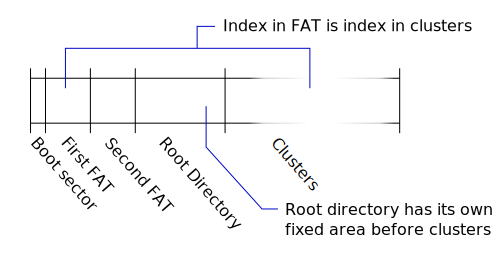
\includegraphics[width=.7\textwidth]{fat16_layout.pdf}
\caption{FAT16 Layout}
\label{fig:fat16_layout}
\end{figure}

\begin{figure}[htb]
\centering
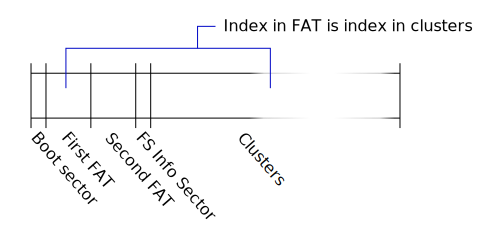
\includegraphics[width=.7\textwidth]{fat32_layout.pdf}
\caption{FAT32 Layout}
\label{fig:fat32_layout}
\end{figure}

FAT16 (and FAT12) have the particularity that the root directory is not like
other directories, but is instead inside its own area preceding the start of
the ``clusters'' area. This also implies that the maximum number of entries in
the root directory is fixed when formatting. FAT32 removes this limitation, and
adds an additional \ac{fsis} containing dynamic information about the state of
the filesystem, e.g. the amount of allocated/free space.

\section{Implementation and Limitations}

We have implemented read-only support for FAT16 and FAT32. However, because the
example \lstinline+ata_rw28+ interface only has the 28-bit {\tt READ DMA} and
{\tt WRITE DMA} commands, we can only access the first 128GB of a disk (with
512-byte sectors).

\subsection{Unicode}

While FAT 8.3 filenames are 8-bit strings, FAT long filenames use UTF-16.
Barrelfish does not have any concept of Unicode, so our FAT implementation
replaces non-\acs{ascii} characters with a question mark in directory listings,
and does not support opening files with non-\acs{ascii} filenames.

\subsection{BSD conv Functions}

To generate 8.3 filenames in the first place, we have adapted various
conversion functions from OpenBSD's msdosfs. However, our current
implementation still compares filenames case-sensitively.

\section{Caching Layer}

\begin{figure}[htb]
\centering
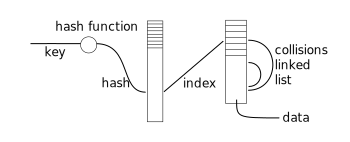
\includegraphics[width=.7\textwidth]{cache_design.pdf}
\caption{Cache Design}
\label{fig:cache_design}
\end{figure}

The FAT code uses a cache layer as a global block and cluster store,
simplifying the code and improving performance. The cache is implemented as a
fixed-size hashmap from keys to indices into a backing array. The backing array
uses doubly linked lists to handle collisions, the free list, and a list of
unused cache entries that can be freed if space is required. Clients must
acquire a reference to a cache entry, either using \lstinline+fs_cache_acquire+
if the entry is already present, or \lstinline+fs_cache_put+ when creating a
new entry. When the entry is no longer used, the client must call
\lstinline+fs_cache_release+. If the reference count for an entry sinks to
zero, it is appended to the aforementioned list of unused entries, which can be
seen as an \acs{lru} queue. Thus when \lstinline+fs_cache_put+ is called and
the cache is at its maximum capacity, it can pop the front entry from the
unused list, free its data, and use the entry for the new cache item.

The caching API consists of the following methods:
\begin{itemize}
	\item \lstinline+fs_cache_init+ and \lstinline+fs_cache_free+, for cache
		setup and teardown. The initialization method takes the maximum capacity
		of the backing array and the hashmap size. Both values must be powers of
		two.
	\item \lstinline+fs_cache_acquire+, for getting a reference to an existing
		entry.
	\item \lstinline+fs_cache_put+, for adding an item to the cache. This also
		increments the reference count as if \lstinline+fs_cache_acquire+ had
		been called.
	\item \lstinline+fs_cache_release+, for releasing a reference to an entry.
\end{itemize}

\section{VFS Interaction}

The mount URI for FAT has the format
\verb@fat<version>://<port>[+<startblock>]@, e.g. \verb@fat32://0+63@, where
{\tt version} is is either 16 or 32, {\tt port} is the \acs{ahci} port of the
device, and the optional {\tt startblock} specifies the offset the first sector
of the filesystem (the boot sector).

Unlike Barrelfish's ramfs, our FAT implementation does not share state between
multiple mounts using \acs{idc}, so with the current \acs{vfs} implementation
mounting a FAT filesystem gives the mounting domain exclusive access to the
filesystem and the whole disk. An alternative that would avoid code duplication
would be for the \acs{vfs} to allow part of its directory structure to be
exported as a service, creating a Barrelfish-internal system conceptually
similar to NFS.


\chapter{Running the AHCI Driver}
This chapter details the ways the \ac{ahci} driver can be 
run and elaborates on the adjustments needed to be able to 
run the driver on real hardware.

\section{QEMU}

Since version 0.14, QEMU contains an emulation layer for an \acs{ich}-9
\ac{ahci} controller\footnote{The QEMU 0.14 changelog is available at
\url{http://wiki.qemu.org/ChangeLog/0.14}}. To define a disk, the QEMU command
line needs to be extended with:

\begin{lstlisting}[language=bash]
 -device ahci,id=ahci -device ide-drive,drive=disk,bus=ahci.0 \
 -drive id=disk,file=/path/to/disk.img,if=none
\end{lstlisting}

QEMU emulates an \acs{ich}-9 controller sufficiently well that little special
code is required. A first workaround is needed for finding the \ac{ahci}
\acs{pci} \ac{bar}; since the QEMU \ac{ahci} emulation layer does not provide
the legacy IDE compatibility mode, the \ac{ahci} MMIO region is found in
\ac{bar} 0 instead of \ac{bar} 5. Another workaround is necessary when
receiving the response for an {\tt IDENTIFY}, which is a PIO command but is
delivered as a Device to Host Register \ac{fis} by QEMU.

\section{Physical Hardware}

Running Barrelfish on real hardware, one can run into several issues. In order
to be able to test our \ac{ahci} implementation, we had to adjust several
aspects of Barrelfish outside the scope of the \ac{ahci} driver infrastructure.
This chapter details any additional modifications.

\subsection{PCI Base Address Registers}

Barrelfish's system knowledge base is not able to handle addresses above 32 bit
correctly. Fixing this issue would require extensive modifications in the
\acs{skb} which are out of the scope of this lab project. As a consequence,
\emph{ahcid} will receive zero \acp{bar} on hardware where the \ac{ahci} memory
regions are mapped in memory above 4GB and thus be unable to access the memory
mapped I/O region to control the \ac{hba}. For the same reason, the code produced by
this lab project has not been tested for 64bit addresses in memory mapped I/O
regions.  Still, once the issues in the \acs{hba} have been fixed, the driver should
properly recognise and handle the devices in question.

\subsection{PCI Bridge Programming}

Because of a bug in \acs{pci} bridge programming, Barrelfish sometimes does not
program \acs{pci} \acp{bar} correctly if \acs{pci} bridges are present. For
this lab project, we introduce a workaround that will retrieve the original
\acp{bar} in case no reprogrammed \acp{bar} can be found in the \acs{skb}.

This is achieved in the \lstinline+device_init+ function of \lstinline+pci.c+,
by querying the \acs{skb} for the original \lstinline+bar(...)+ facts of the
device if no reprogrammed ones can be found:

\begin{lstlisting}
error_code = skb_execute_query(
  "findall(baraddr(BAR,Base,0,Size),bar(addr(%u,%u,%u)"
  ",BAR,Base,Size,_,_,_), BARList),"
  "sort(1, =<, BARList, L),"
  "length(L,Len),writeln(L)",
  *bus, *dev, *fun);
\end{lstlisting}

The result of this prolog expression has exactly the same form as
\lstinline+pci_get_+\linebreak \lstinline+implemented_BAR_addresses+ therefore
the surrounding code is exactly the same as in the usual case.

\subsection{BIOS Memory Maps}

On x86 architectures, the BIOS memory map can be retrieved to determine the
layout of memory. Some BIOSs report a memory map that is not sorted by
increasing base address or even might return overlapping and conflicting memory
regions.  This lab project contains modifications to the code that creates
capabilities to physical memory in \verb+startup_arch.c+ such that the memory
map is preprocessed to eliminate conflicts and ensure ascending addresses.

As the preprocessed memory map might be larger due to the case where one memory
region completely contains another and thus is split into three new regions, we
first need to copy the map into a larger buffer. The memory map is then sorted
with a simple bubblesort.  To remove conflicts, overlapping regions are given
to the region with the higher type or merged if they are both of the same type.
At the end, regions are page-aligned as Barrelfish can only map whole pages.

\autoref{fig:mmap} shows the memory maps seen on a DELL Optiplex 755
workstation. Several regions are not aligned to the pagesize and the region at
\lstinline+0xfec00000+ does not appear in ascending order. After preprocessing,
memory addresses appear in ascending order and are page-aligned. Note that
higher types take precedence, therefore page alignment does not necessarily
round down.

\begin{figure}[ht]
\centering
\includegraphics[width=.7\textwidth]{mmap.pdf}
\caption{Memory map transformation}
\label{fig:mmap}
\end{figure}


\chapter{Future Work}
\section{ATA Messages}

Since this lab project was geared towards designing and implementing a message
passing interface to disk, only very few message types have been defined to
showcase the interface. \ac{sata} supports a wider range of devices which can
benefit from more aspects of the \ac{ata} command set, such as {\tt TRIM} on
solid state drives. Adding further commands to the flounder-based approach is
as simple as adding a further message definition.

\section{Integration with the System Knowledge Base}

As we have mainly focused on getting message passing to disk to work, we have
taken a few shortcuts concerning the integration of our subsystem into
Barrelfish as a whole. For instance, we do not really use the \acs{skb} to
uniquely identify the disks attached to an \ac{ahci} controller.  Neither do we
use the \acs{skb} to store additional data, e.g. serial number and size, of the
attached disks. Adding that kind of data would simplify discovery of disks and
acting appropriately, for example automatically mounting a volume or similar.

\section{Handling multiple AHCI controllers at the same time}

Currently our management daemon (see \longref{chap:ahcid}) successfully exits
from the initialization code as soon as a \ac{ahci} controller has been found.
It would be prefereable if on systems with multiple controllers attached all of
these could be used. One consideration in this case would be whether to have
one management daemon per controller or a global management daemon that
controls all available \ac{ahci} controllers.

\section{Support for advanced AHCI/SATA features}

Some of the features of \ac{ahci}/\ac{sata} we did not look at are Port
Multiplication and \ac{ncq}.

However, our system design, including a management daemon that presents each
port to the rest of the system as a separate entity, makes accomodating
multiplied ports (multiplying ports is actually done in hardware and the
\ac{ahci} host controller has a register for each port which contains the port
multiplication status for that port) relatively easy as the only parts that
have to be changed are the management daemon and libahci. Also, \ac{ncq} could
be implemented almost entirely in libahci, if desired.

We also do not handle hotplug of devices. Addition of devices could implemented
relatively easy by extending ahcid's interrupt handler and performing the
initialization steps once the link to the device has been established. Removal
however is more challenging. Outstanding requests have to be completed with an
error, the user notified and memory resources reclaimed.

\section{Further Controllers}

The modular nature of the Flounder-based approach allows to add additional
backends for other controllers. Since this lab project only examined
\ac{ahci}-compliant controllers, support is limited to realtively new
controllers for \ac{sata}. In reality, there are still a lot of use cases where
one might have to access \ac{pata}-based devices, such as older CDROM drives.
Therefore, backends for more chipsets should be developed, most importantly one
for a widespread \ac{pata} controller such as the \acs{piix} family or the
\acs{ich} controllers before the introduction of \ac{ahci}.


\chapter{Conclusion}
In the course of this lab project we successfully implemented an \ac{ahci}
driver and supporting code for data storage and retrieval.

\section{Flounder Modifications}

The extensions added to flounder provide a very simple and extensible way to
interface with disks. The overhead incurred is acceptable in the trade-off for
simplicity and modularity. The seperation of interface definition for \ac{ata}
from implementation of command dispatching to the device allows simple addition
of further \ac{ata} transports, such as additional \acs{pata}/\acs{sata}
controllers.

\section{Security}

The \acs{ahci} driver demonstrates the trade-off when dealing with \acs{dma}.
If a domain is allowed full control over the configuration of \acs{dma}
aspects, it can obtain full read/write access to physical memory. To mitigate
this problem, the management service would have to check and validate any
memory regions supplied before allowing a command to execute. If only trusted
domains are allowed to bind to the \acs{ahci} driver, these checks are not
neccessary. This is a valid assumption, as filesystems and blockdevice-like
services are the only ones that should be allowed raw access to disks.

\section{Performance}

Performance is in the same order of magnitude as seen on Linux for large
blocksizes and random access. There is some bottleneck during read operations
that could relate either to interrupt dispatching or memcopy performance.  To
achieve high throughput on sequential workloads with small blocksizes, a
prefetcher of some sort is necessary. A possible solution would be to have a
cache that stores pages or larger chunks of data. A read operation would then
have to read multiples of the cached size if the data is not present in the
cache. If data is cached, the request can be completed much faster without
needing to consult the disk.


\cleardoublepage
\phantomsection
\addcontentsline{toc}{chapter}{Bibliography}
\bibliographystyle{plain}
\bibliography{references}

\appendix

%\chapter{Glossary}
\phantomsection
\printglossaries

\end{document}
